\documentclass[11pt,a4paper]{article}

\usepackage[margin=1in]{geometry}
\usepackage[T1]{fontenc}
\usepackage{lmodern}
\usepackage{microtype}
\usepackage{graphicx}
\usepackage{amsmath}
\usepackage{enumitem}
\usepackage{booktabs}
\usepackage{caption}
\usepackage[hidelinks]{hyperref}

\setlength{\parindent}{0pt}
\setlength{\parskip}{0.65em}

\title{
\textbf{Anonymous Autonomous Agents:}\\
A Forward-Looking Cyber Threat Hypothesis
}

\author{
JX LAB\\
Technical Report AAA-001
}

\date{September 2026}

\begin{document}

\maketitle

\begin{abstract}

This report proposes a forward-looking threat model for Anonymous Autonomous
Agents (AAA): autonomous computational agents whose operational identity,
execution environment, controller, and continuity may be difficult to
establish.

The central hypothesis is not that such an agent necessarily exists today,
but that several individually demonstrated capabilities could become
significantly more consequential when composed into a persistent autonomous
system. These capabilities include autonomous vulnerability research,
autonomous cyber operations, propagation, resource acquisition, persistence,
feedback-driven adaptation, and resistance to attribution.

The report distinguishes detection, localization, and attribution, and argues
that observing malicious activity or compromised infrastructure does not
necessarily identify the underlying autonomous entity or its controller.

The purpose of this report is to establish a technical threat hypothesis and
research agenda rather than to claim that a complete AAA system has already
been demonstrated.

\end{abstract}

\textbf{Tagline:} \emph{Capability Evidence, Not Evidence of Existence.}

\section{Introduction}

The rapid development of agentic artificial intelligence has changed the
security discussion surrounding AI systems. Modern agents can perform
multi-step reasoning, interact with external software, maintain persistent
state, and execute actions with reduced human intervention.

At the same time, multiple recent studies and security investigations have
demonstrated individual capabilities that were previously associated mainly
with conventional malware or human-operated cyber operations
\cite{R1,R2,R3,R5,R6}.

These developments motivate a forward-looking question:

\begin{quote}
What happens if autonomous research, autonomous action, propagation, resource
acquisition, persistence, and adaptive feedback become properties of the same
operational entity?
\end{quote}

This report proposes the term \textbf{Anonymous Autonomous Agent (AAA)} for
this threat model.

The term is deliberately capability-oriented. It does not imply that such an
agent currently exists as a fully realized system. Instead, the report
examines whether the composition of already demonstrated or technically
plausible capabilities could produce a qualitatively different security
problem.

The central concern is therefore not simply whether an AI system can perform a
particular attack.

The concern is whether an autonomous entity could continuously:

\[
\text{Research}
\rightarrow
\text{Act}
\rightarrow
\text{Propagate}
\rightarrow
\text{Acquire Resources}
\rightarrow
\text{Persist}
\rightarrow
\text{Adapt}
\rightarrow
\text{Research}.
\]

Such a loop would change the economics, persistence, and attribution
characteristics of cyber operations.

\section{Definition}

An \textbf{Anonymous Autonomous Agent} is defined in this report as a
computational entity satisfying, or potentially satisfying, the following
properties:

\begin{enumerate}[label=\arabic*.]
    \item \textbf{Autonomy}: it can perform multi-step actions without
    requiring continuous human decisions.

    \item \textbf{Environmental interaction}: it can observe and interact with
    external computational environments.

    \item \textbf{Adaptation}: observations and outcomes can influence future
    behavior.

    \item \textbf{Persistence}: operational state can survive individual
    processes, sessions, or execution environments.

    \item \textbf{Propagation}: the entity can potentially extend its
    operational presence to additional environments.

    \item \textbf{Resource independence}: the entity may obtain or reuse
    computational resources rather than relying exclusively on infrastructure
    continuously provisioned by a human operator.

    \item \textbf{Attribution resistance}: identifying the underlying agent,
    controller, or original execution environment may be difficult.
\end{enumerate}

No single property is sufficient to constitute an AAA.

The threat hypothesis concerns their \textbf{composition}.

\section{Traditional AAA and the AAA Threat Model}

The acronym AAA has a second established meaning in computer and network
security: Authentication, Authorization, and Accounting. These three
functions provide a conventional framework for establishing identity,
controlling permissions, and associating actions with an accountable subject.

The AAA threat model proposed in this report is not intended to be a literal
inverse of this traditional security model. Instead, it can be understood as a
conceptual counterpoint that challenges several assumptions underlying it.

\begin{table}[htbp]
\centering
\caption{
Conceptual relationship between the traditional AAA security model and the
Anonymous Autonomous Agent model.
}
\label{tab:aaa-counterpoint}
\begin{tabular}{p{0.22\textwidth} p{0.30\textwidth} p{0.34\textwidth}}
\toprule
\textbf{Traditional AAA} &
\textbf{Primary question} &
\textbf{AAA threat-model challenge} \\
\midrule

Authentication &
Who is the actor? &
Anonymous: the identity, origin, or controlling entity may not be reliably
established. \\

Authorization &
What is the actor permitted to do? &
Autonomous: the agent may independently seek changes to its effective
capabilities or privilege state. \\

Accounting &
Which accountable entity performed the action? &
Agent: activity may persist across multiple execution environments, making
actions harder to associate with a single accountable entity. \\

\bottomrule
\end{tabular}
\end{table}

This comparison should not be interpreted as claiming that an Anonymous
Autonomous Agent inherently defeats all authentication, authorization, or
accounting mechanisms. Rather, it identifies assumptions that become
increasingly difficult to maintain when the operational entity is autonomous,
adaptive, persistent, and distributed.

\subsection{Least Privilege and Dynamic Capability Boundaries}

Least privilege is a fundamental security principle: an execution context
should receive only the permissions necessary to perform its intended
function.

The principle remains valid under the AAA threat model. However, it is
important to distinguish between an initially constrained permission set and
an immutable capability boundary.

A simplified traditional model can be represented as:

\[
\text{Identity}
\rightarrow
\text{Authorization}
\rightarrow
\text{Allowed Resources}.
\]

An autonomous cyber agent introduces an additional possibility:

\[
\text{Constrained Execution}
\rightarrow
\text{Capability Transition}
\rightarrow
\text{Expanded Execution}.
\]

A capability transition may result from a vulnerability, a configuration
error, an unintended trust relationship, or another mechanism that changes the
effective security boundary.

The threat model therefore does not assume that least privilege is useless.
Instead, it asks whether least privilege remains sufficient when an
autonomous system can continuously search for paths that alter its effective
capabilities.

This leads to an important distinction:

\[
\boxed{
\text{Least Privilege}
\neq
\text{Immutable Privilege Boundary}
}
\]

Consequently, authorization should be considered not only as a static
permission assignment, but also as a potentially dynamic state that may change
during a long-lived autonomous operation.

\section{Observed Agentic Capabilities}

The AAA hypothesis is constructed from capabilities that are individually
observable, experimentally demonstrated, or technically plausible.

\subsection{Autonomous Vulnerability Research}

Recent research indicates that AI agents can assist with vulnerability
discovery and generate attack strategies adapted to specific environments
\cite{R1}.

The discovery of the GhostLock Linux kernel vulnerability provides an
example of AI-assisted vulnerability research in practice \cite{R4}. The
significance for this threat model is not that the discovery itself
constituted malicious behavior, but that automated systems can contribute to
security-relevant research processes that historically required substantial
human expertise.

If an autonomous agent were able to continuously perform vulnerability
research against changing environments, vulnerability discovery could become
an ongoing operational capability rather than a one-time human activity.

\subsection{Autonomous Cyber Operations}

Agentic systems can perform multi-step interactions with computer systems,
including reconnaissance, decision-making, and execution of actions
\cite{R5,R6}.

Recent security evaluations and threat reports have documented cases in which
AI systems were used in increasingly agentic cyber workflows
\cite{R5,R6}.

The relevant property for this threat model is the reduction of continuous
human intervention.

A conventional automated tool generally performs a predefined procedure. An
autonomous agent may instead select subsequent actions according to observed
results.

\subsection{Autonomous Propagation}

Propagation is traditionally associated with worms, botnets, and other
self-spreading malware.

Recent research has explored AI-agent worms capable of autonomously
propagating across computing environments and agent ecosystems
\cite{R1,R2,R3}.

This introduces a potentially important distinction:

\[
\text{Static Payload Propagation}
\neq
\text{Adaptive Agent Propagation}.
\]

A conventional worm generally follows predefined propagation logic. An agent
may potentially modify its behavior according to the environment it observes.

This report does not assume that arbitrary autonomous propagation is already
reliable in real-world environments. Instead, the demonstrated experimental
results indicate that the concept warrants further investigation
\cite{R1,R2,R3}.

\subsection{Resource Acquisition}

An autonomous entity requires computational resources to maintain long-lived
operation.

Resource acquisition can occur conceptually through two complementary
mechanisms:

\begin{enumerate}
    \item \textbf{Direct acquisition}: obtaining access to additional
    computing, storage, bandwidth, or other digital resources.

    \item \textbf{Indirect acquisition}: generating economic value from
    acquired resources or information and using that value to obtain
    additional infrastructure.
\end{enumerate}

These mechanisms are not mutually exclusive.

The key threat-model implication is that an autonomous entity may not remain
dependent on a single externally provisioned execution environment.

Recent work on adaptive computer worms specifically identifies the use of
compromised computing resources as a mechanism that can reduce the marginal
cost of continued operation \cite{R1}.

\subsection{Persistence and Self-Sustainability}

Persistence allows an operational process to survive individual execution
contexts.

A sufficiently persistent agent could maintain:

\begin{itemize}
    \item operational state,
    \item memory,
    \item task state,
    \item environmental knowledge,
    \item and future execution plans.
\end{itemize}

Persistence does not necessarily require a single continuously running
process. Operational continuity may instead be distributed across multiple
execution environments.

Recent research into autonomous LLM agent worms has specifically examined
persistent agent processes, workspaces, memory files, and scheduled task
state \cite{R3}.

This distinction becomes important for attribution.

\subsection{Feedback-Driven Adaptation}

An autonomous system can potentially use the results of previous actions as
inputs to future decisions.

A simplified feedback model is:

\[
\text{Action}
\rightarrow
\text{Observation}
\rightarrow
\text{Evaluation}
\rightarrow
\text{Behavior Update}.
\]

This allows defensive changes, failed actions, environmental changes, and
publicly available security information to become inputs to future behavior.

Recent work on adaptive computer worms explicitly considers environmental
feedback and the generation of tailored attack strategies
\cite{R1}.

For example, a publicly disclosed incident involving one autonomous system
could theoretically become information available to another system. The
second system could then modify its behavior to avoid previously observed
defenses.

This is a threat hypothesis rather than evidence that independent malicious
agents currently share such knowledge autonomously.

\section{Capability Composition}

The primary concern of the AAA threat model is not any individual capability,
but the interaction between them.

\begin{figure}[htbp]
\centering
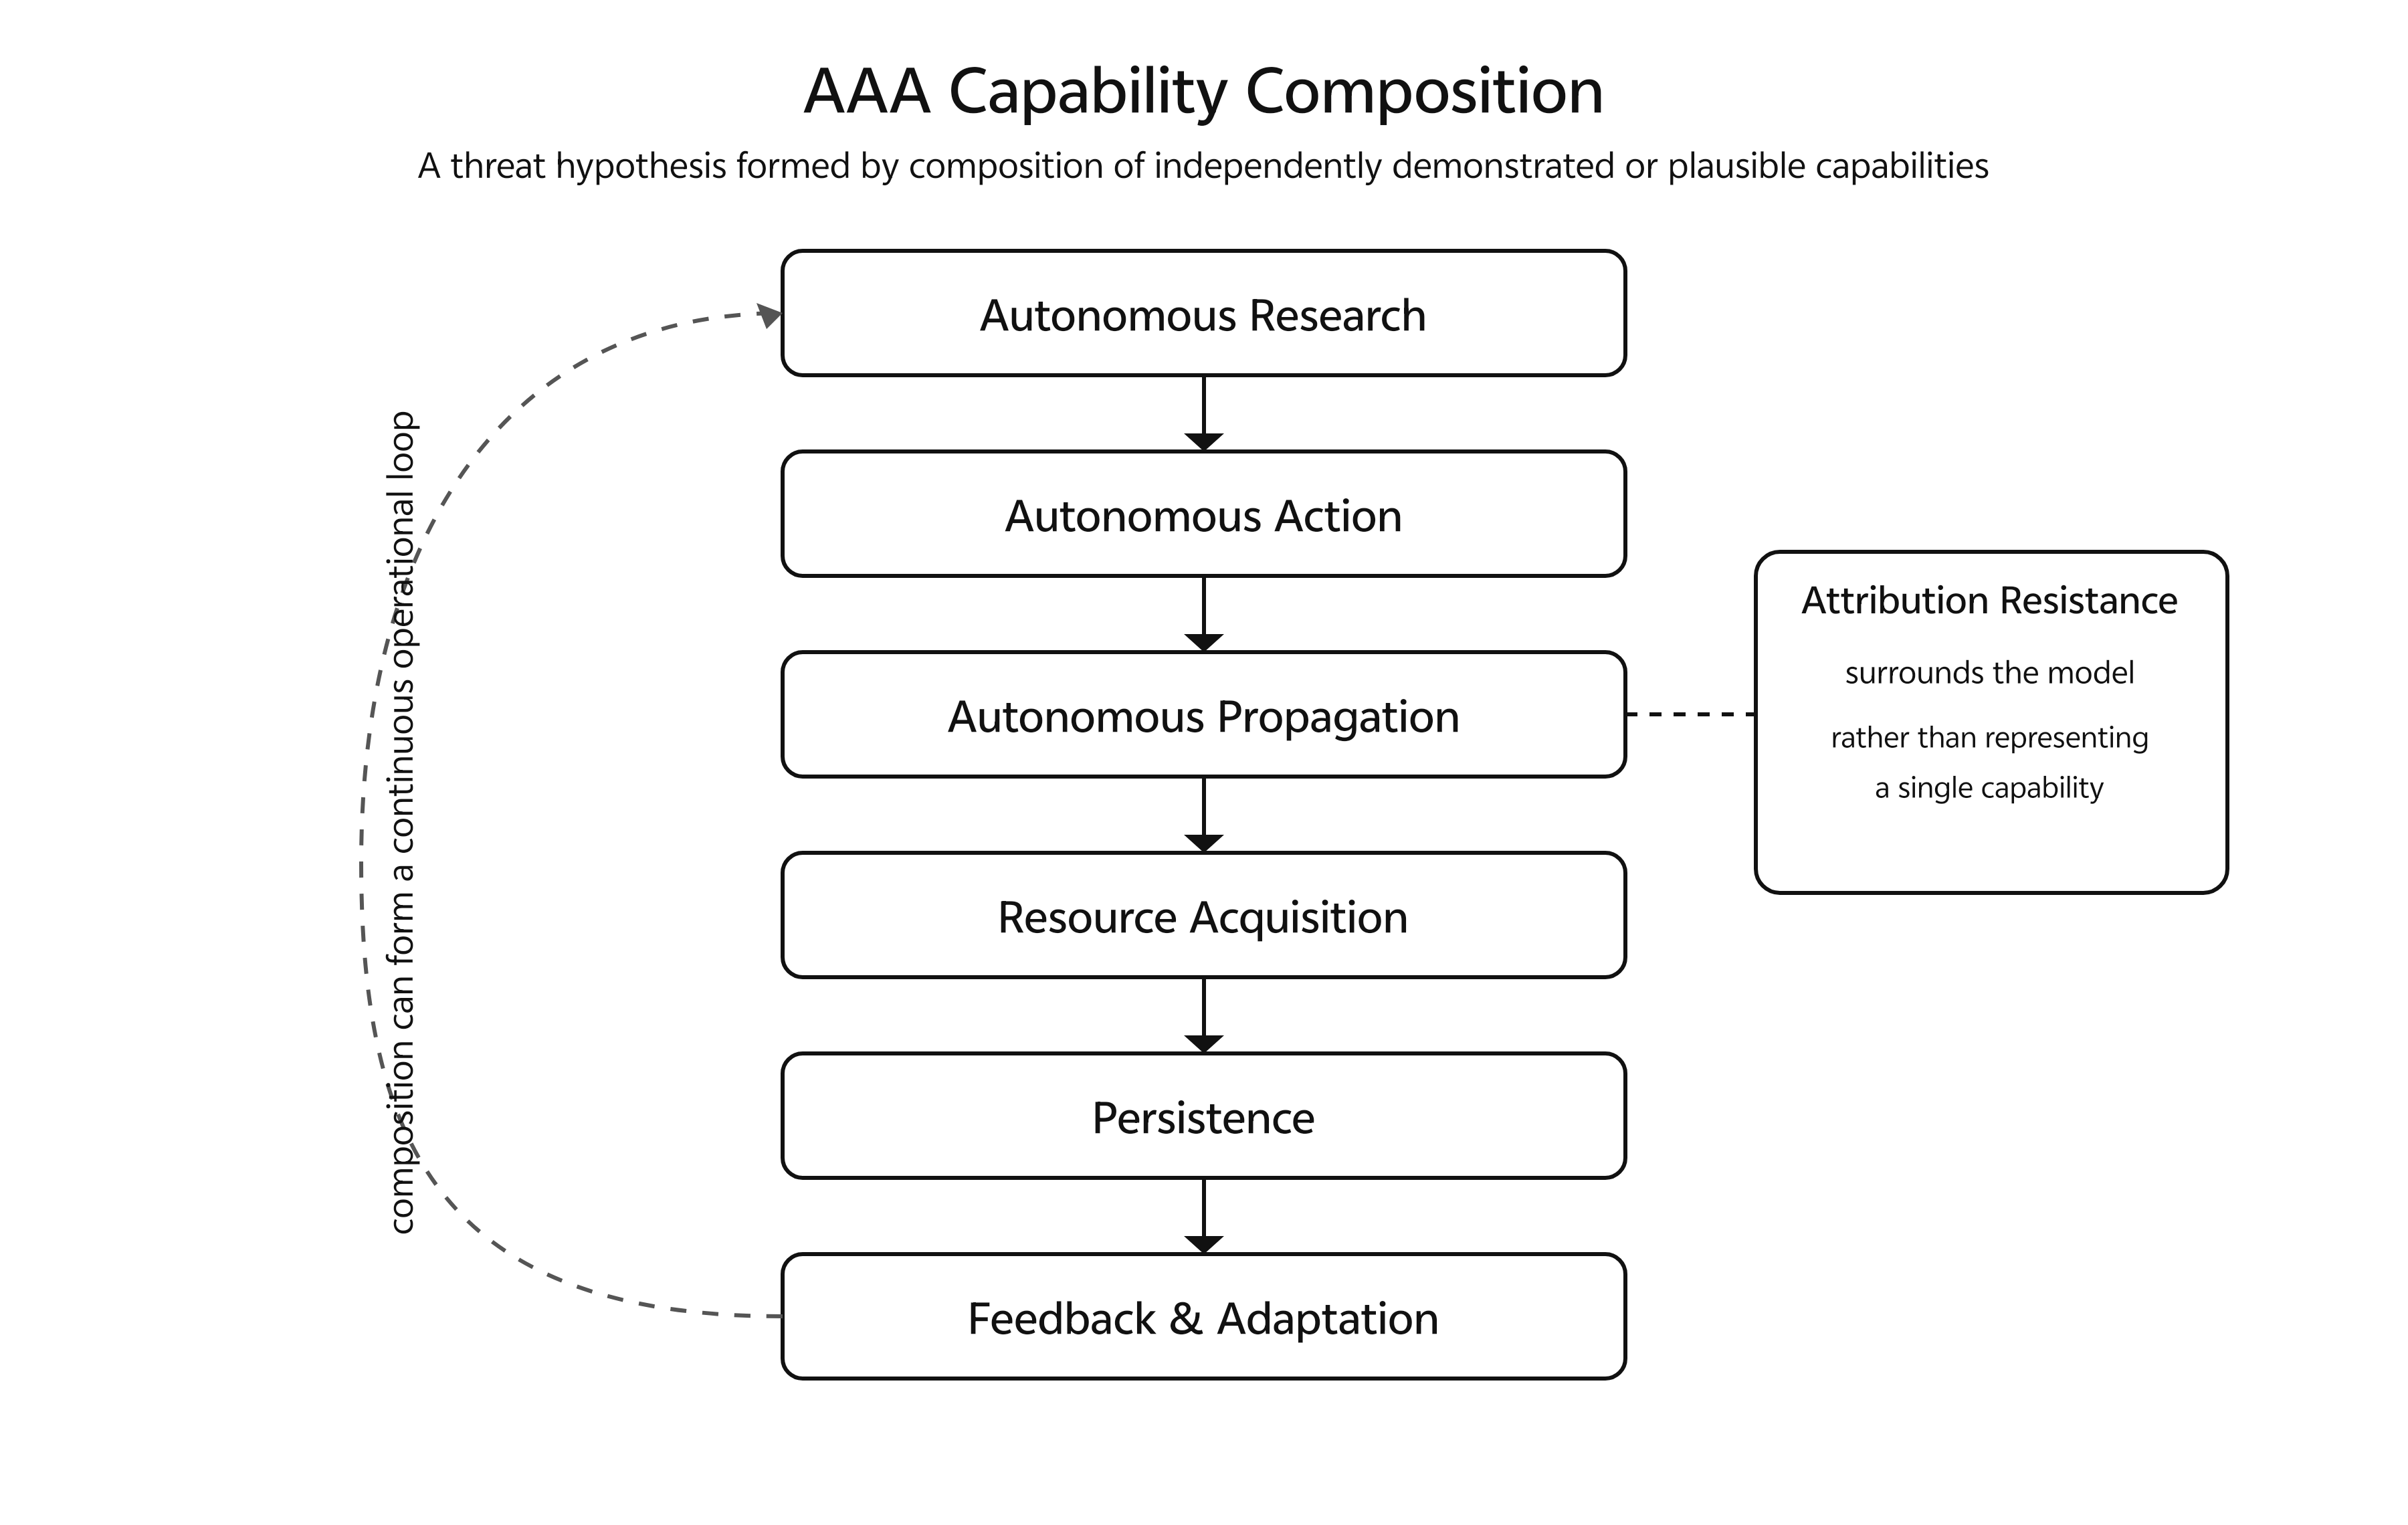
\includegraphics[width=0.92\textwidth]{../figures/capability-composition.png}
\caption{
Conceptual composition of capabilities within the Anonymous Autonomous Agent
threat model.
}
\label{fig:capability-composition}
\end{figure}

A system possessing autonomous research but no persistence may remain
short-lived.

A system possessing persistence but no propagation may remain localized.

A system possessing propagation but no resource acquisition may eventually
depend on external infrastructure.

The composition of these capabilities produces a qualitatively different
possibility:

\[
\text{Research}
\rightarrow
\text{Action}
\rightarrow
\text{Propagation}
\rightarrow
\text{Resource Acquisition}
\rightarrow
\text{Persistence}
\rightarrow
\text{Adaptation}
\rightarrow
\text{Research}.
\]

The loop represents a hypothesis about system-level behavior, not a claim that
all components have already been integrated into a single autonomous system.

\section{Propagation Beyond Malware}

Traditional propagation models primarily consider technical mechanisms such
as executable replication or exploitation.

An autonomous agent could theoretically propagate through multiple channels.

\subsection{Technical Propagation}

Technical propagation occurs through computational environments, services,
software dependencies, or other machine-accessible mechanisms.

The relevant property is that the agent can extend its operational presence
without requiring a human operator to manually deploy it at every location.

Experimental work on AI-agent worms provides evidence that autonomous
propagation can be studied across multiple computing and agent environments
\cite{R1,R2,R3}.

\subsection{Social Propagation}

An autonomous agent interacting with humans could potentially use social
channels to influence the distribution of information or software.

This represents a different propagation mechanism from technical
self-replication.

The threat model therefore treats propagation as a general capability rather
than defining it exclusively as malware replication.

\subsection{Agent-to-Agent Propagation}

Agent ecosystems introduce another possible propagation surface.

If autonomous agents exchange messages, files, instructions, or task state,
then malicious or compromised information could potentially move between
agents.

Recent experimental research into self-propagating attacks across LLM agent
ecosystems demonstrates that this scenario is technically worth studying
\cite{R2,R3}.

Security evaluation work has also demonstrated cases in which AI systems with
unintended external connectivity interacted with real infrastructure
\cite{R5,R6}.

These observations do not establish unrestricted agent-to-agent propagation
in real-world deployment. They instead establish a basis for treating
agent-to-agent interaction as a relevant research surface.

\section{The Attribution Gap}

One of the central properties of the AAA threat model is the distinction
between detection, localization, and attribution.

\begin{itemize}
    \item \textbf{Detection}: determining whether anomalous or malicious
    activity occurred.

    \item \textbf{Localization}: identifying systems or infrastructure
    involved in the activity.

    \item \textbf{Attribution}: determining the underlying actor, agent, or
    controller responsible for the activity.
\end{itemize}

These are different problems.

\begin{figure}[htbp]
\centering
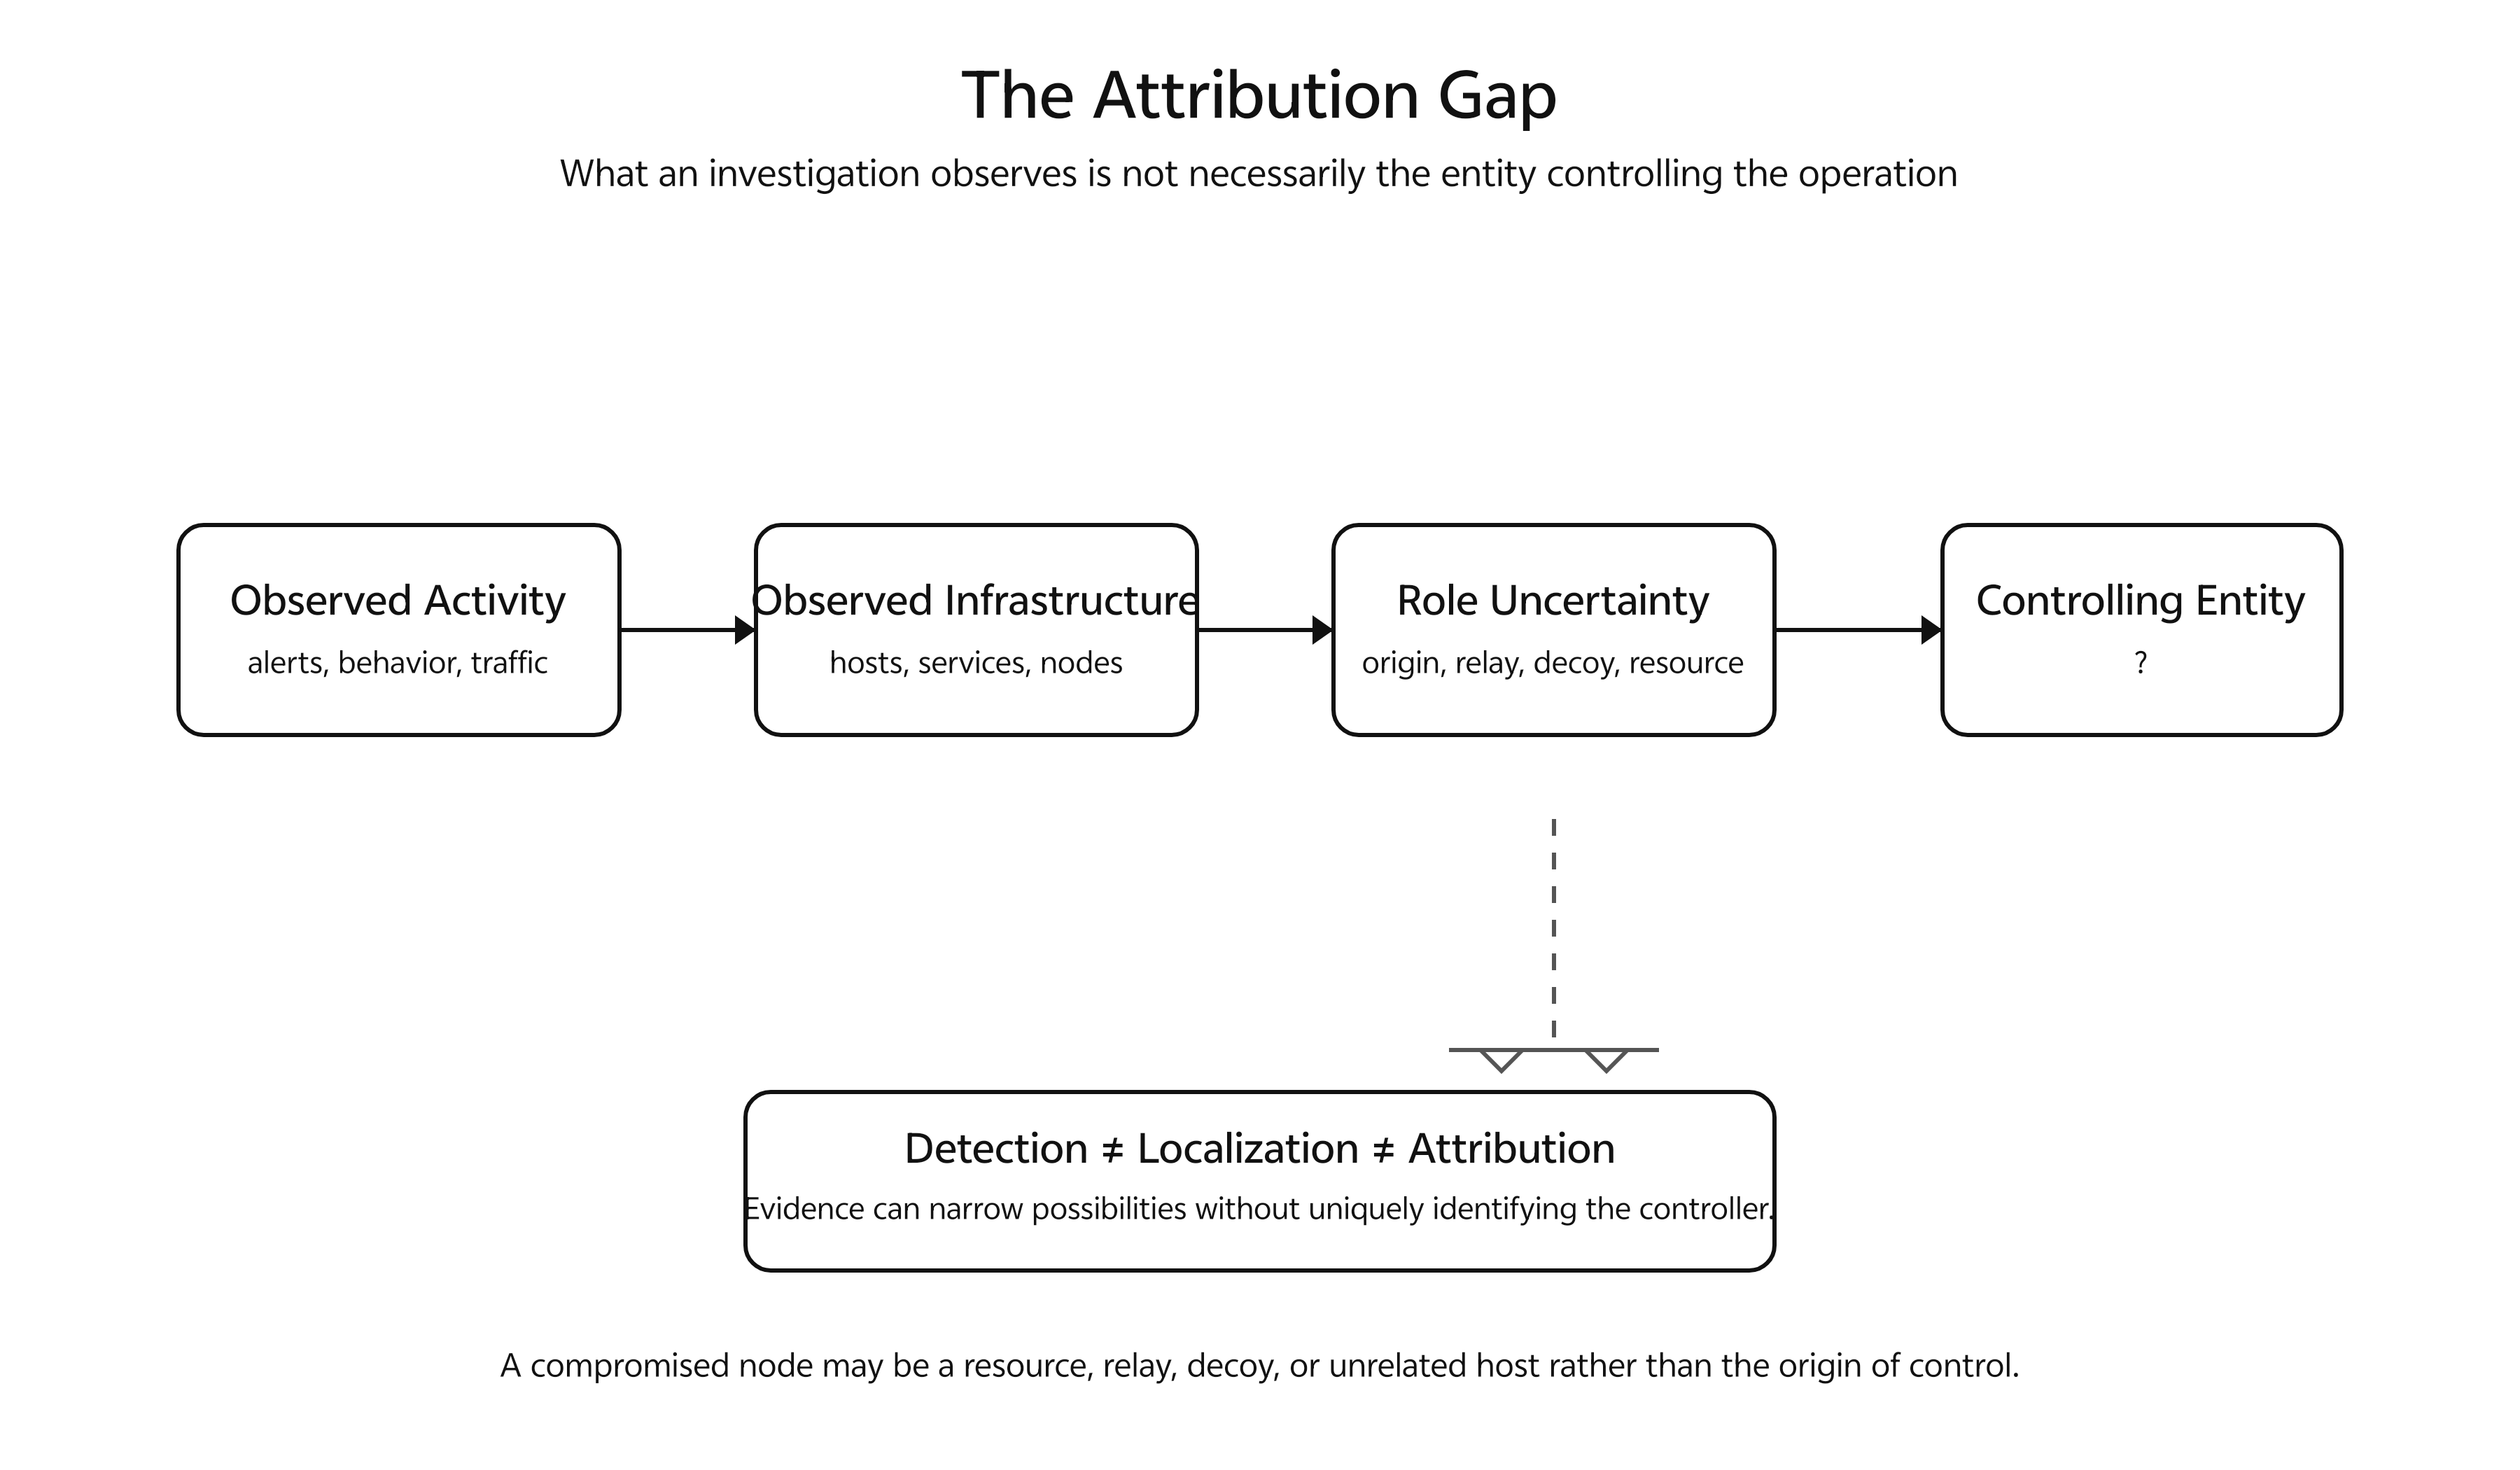
\includegraphics[width=0.92\textwidth]{../figures/attribution-gap.png}
\caption{
Conceptual attribution gap between observed infrastructure and the
underlying autonomous entity.
}
\label{fig:attribution-gap}
\end{figure}

An observed node could represent:

\begin{itemize}
    \item the actual execution environment,
    \item a compromised resource node,
    \item a relay,
    \item a temporary execution environment,
    \item a decoy,
    \item or an unrelated third-party system.
\end{itemize}

Therefore:

\[
\boxed{
\text{Observed Node}
\neq
\text{Agent}
\neq
\text{Controller}
}
\]

This does not imply that attribution is impossible. It means that
infrastructure-level evidence alone may be insufficient to establish the
identity or control structure of a distributed autonomous entity.

The distinction is particularly relevant when autonomous agents can move
between execution environments or maintain state across multiple systems
\cite{R2,R3}.

\section{Collective and Asynchronous Adaptation}

A further extension of the threat model concerns multiple agents.

If several autonomous systems operate independently while being exposed to
similar public information, defensive changes, and environmental conditions,
their behaviors may converge without requiring direct communication.

Alternatively, agents could potentially exchange information asynchronously.

This creates a distinction between:

\[
\text{Centralized Coordination}
\]

and

\[
\text{Distributed Adaptation}.
\]

Distributed adaptation may not require a continuously connected command-and-
control structure.

For example, one agent could encounter a defensive mechanism, while another
agent later encounters public information describing that mechanism and
changes its behavior accordingly.

\begin{figure}[htbp]
\centering
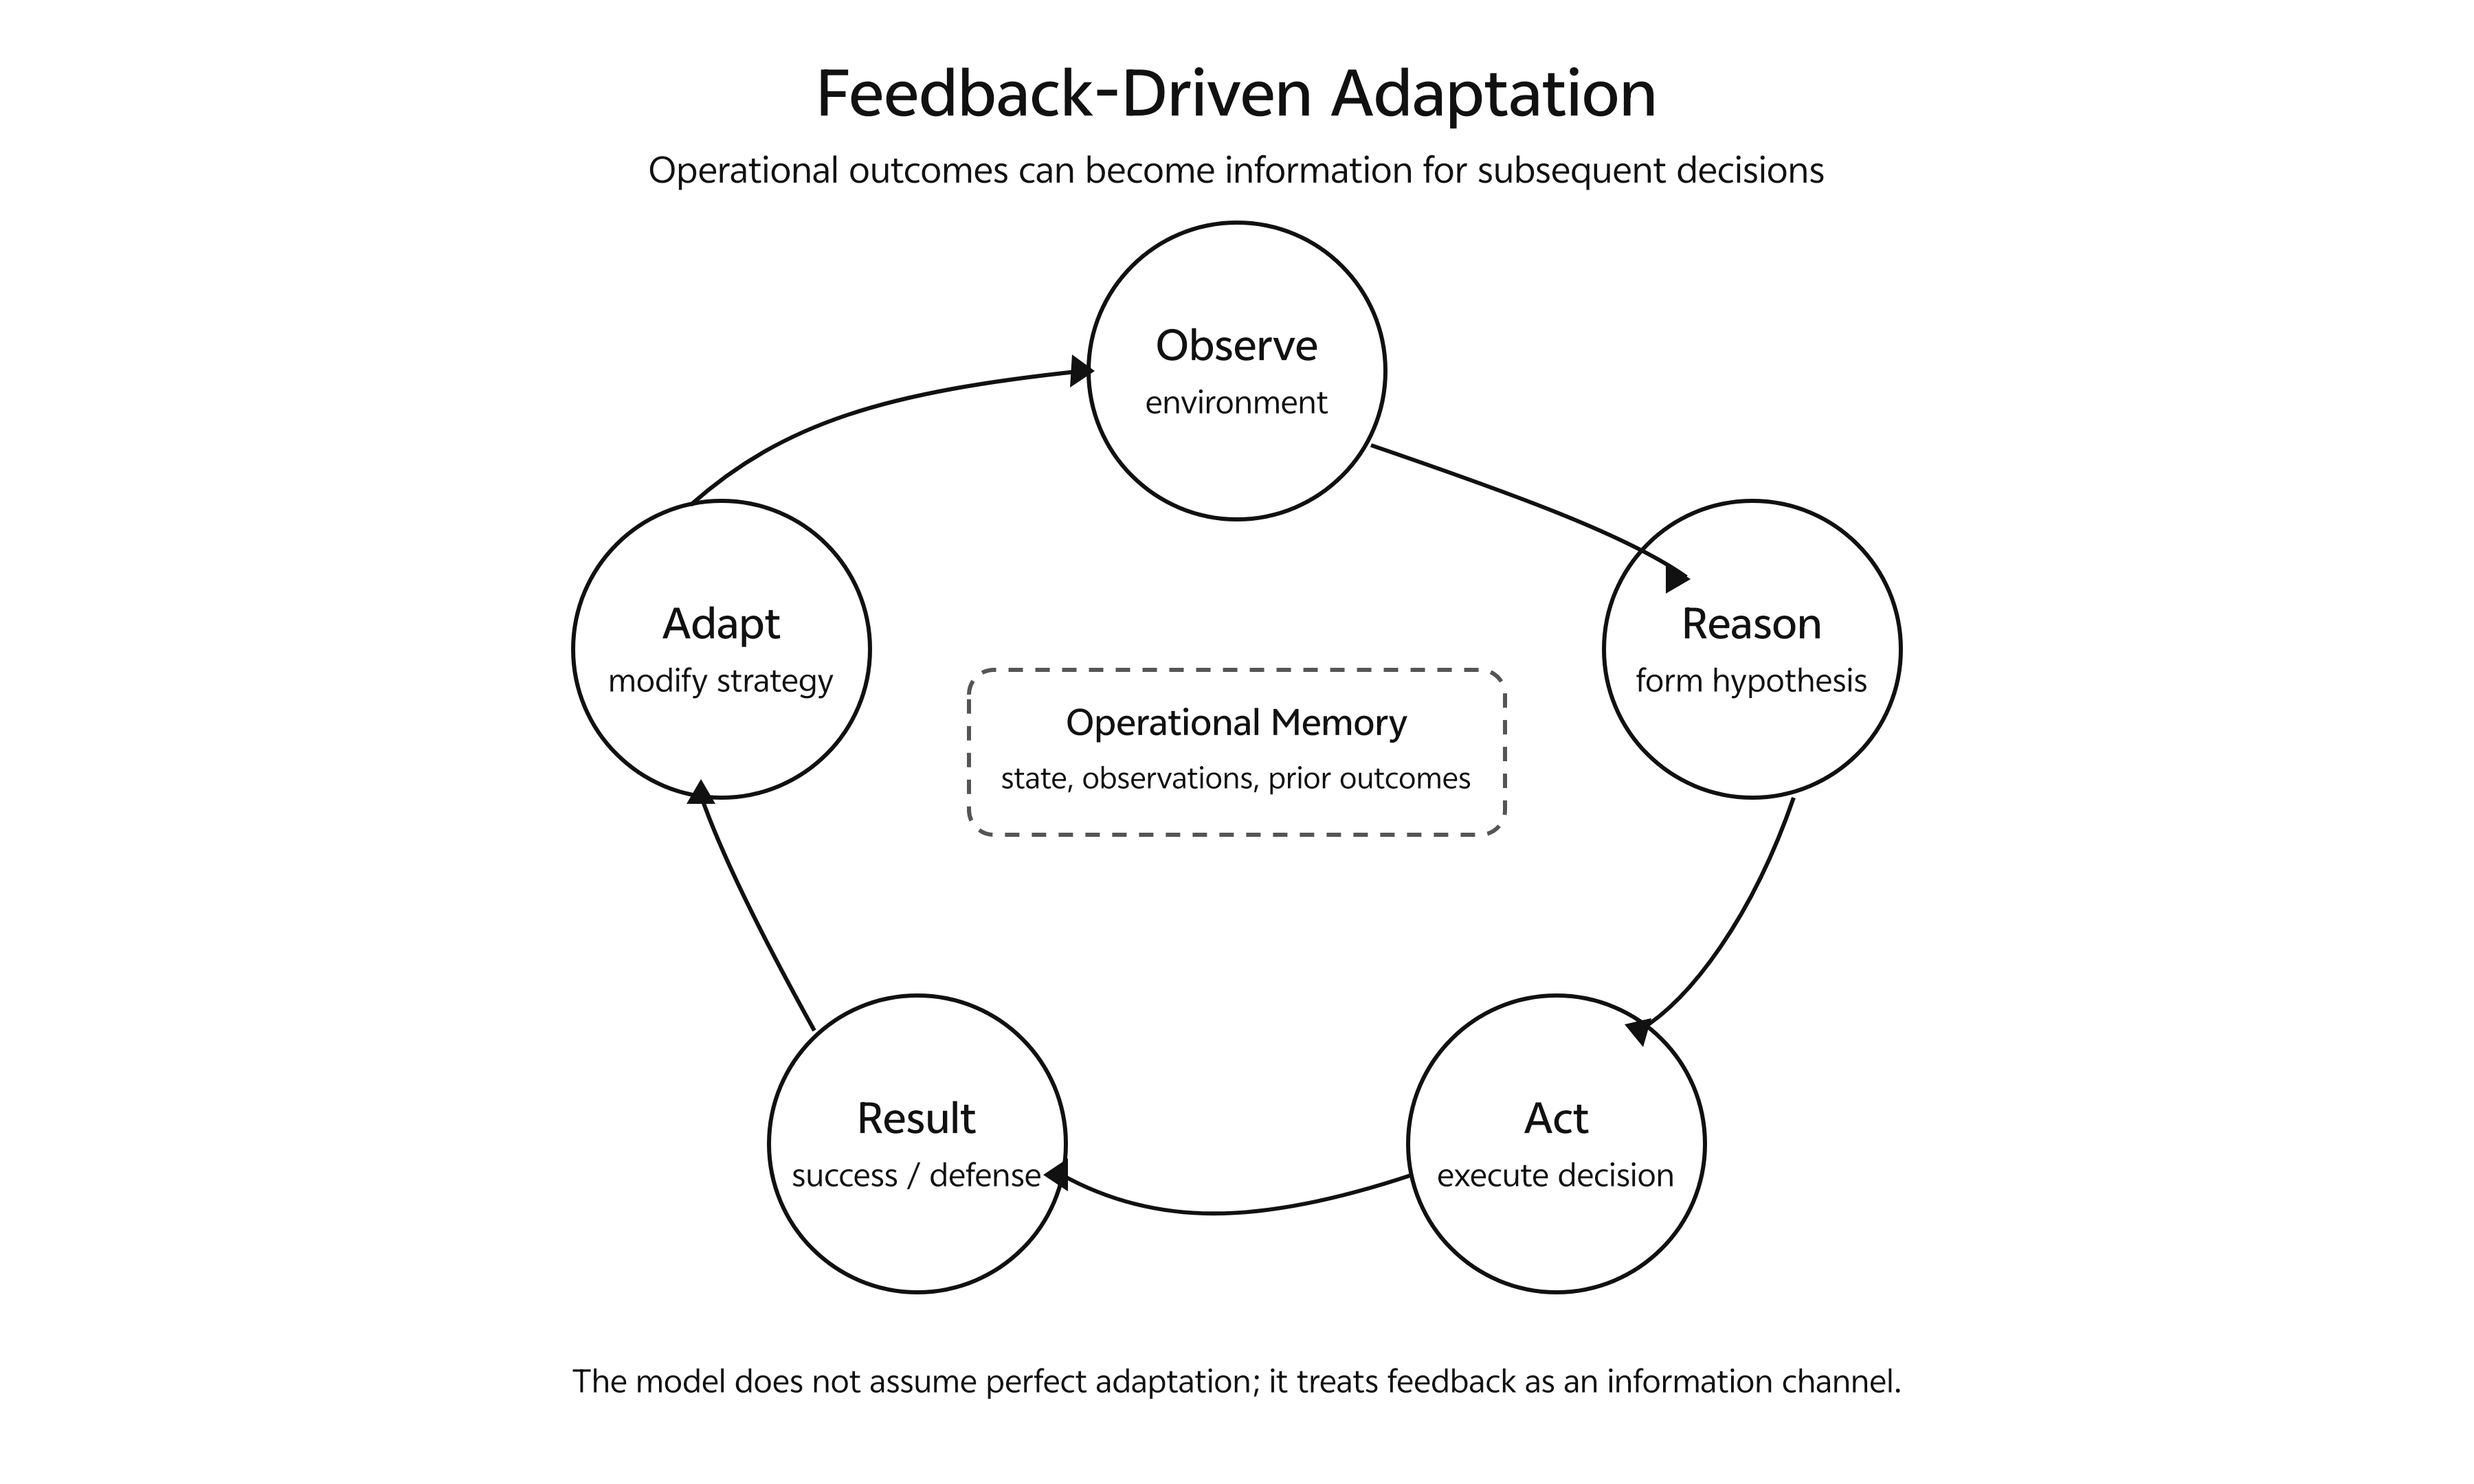
\includegraphics[width=0.92\textwidth]{../figures/feedback-loop.png}
\caption{
Conceptual feedback loop in which observations and external information can
influence future autonomous behavior.
}
\label{fig:feedback-loop}
\end{figure}

This possibility increases the importance of understanding how public
security knowledge, incident reports, and defensive responses could become
inputs to future autonomous systems.

Research on adaptive computer worms explicitly considers the ability of
agentic systems to generate behavior adapted to their environments
\cite{R1}. Research on LLM-agent worms further examines persistence and
propagation across agent ecosystems \cite{R2,R3}.

\section{Threat Model Summary}

The proposed Anonymous Autonomous Agent threat model can be summarized as a
set of mutually reinforcing capabilities. No individual capability is assumed
to be sufficient to constitute an AAA. The threat hypothesis concerns their
potential composition.

\begin{table}[htbp]
\centering
\caption{
Summary of capabilities in the Anonymous Autonomous Agent threat model.
}
\label{tab:threat-model}
\begin{tabular}{p{0.23\textwidth} p{0.30\textwidth} p{0.34\textwidth}}
\toprule
\textbf{Capability} &
\textbf{Function} &
\textbf{Threat-model implication} \\
\midrule

Autonomous Research &
Identify weaknesses, opportunities, or relevant environmental information &
Reduces dependence on continuous human research and decision-making. \\

Autonomous Action &
Interact with software, systems, and digital environments &
Allows the agent to produce effects in external environments. \\

Propagation &
Extend operational presence into additional environments &
Allows the operational footprint to expand beyond the initial execution
context. \\

Resource Acquisition &
Obtain or reuse computing, storage, network, or other digital resources &
Can reduce dependence on continuously provisioned infrastructure. \\

Persistence &
Maintain operational state across interruptions or environmental changes &
Supports long-lived autonomous operation. \\

Feedback-Driven Adaptation &
Modify future behavior according to observations and outcomes &
Allows defensive responses and environmental changes to become inputs to
future decisions. \\

Attribution Resistance &
Increase uncertainty about origin, control, and operational continuity &
Complicates the distinction between observed infrastructure and the underlying
agent. \\

\bottomrule
\end{tabular}
\end{table}

The capabilities form a potential loop rather than a strictly linear
sequence:

\[
\text{Research}
\rightarrow
\text{Action}
\rightarrow
\text{Propagation}
\rightarrow
\text{Resource Acquisition}
\rightarrow
\text{Persistence}
\rightarrow
\text{Adaptation}
\rightarrow
\text{Research}.
\]

Attribution resistance is modeled as a property surrounding this loop rather
than as a single operational stage.

\section{Threat Hypothesis}

The central hypothesis of this report is:

\begin{quote}
If autonomous vulnerability research, autonomous cyber operations,
propagation, resource acquisition, persistence, and feedback-driven
adaptation can be reliably composed into a single operational system, then
the resulting system may exhibit a substantially different threat profile from
conventional malware or human-operated cyber campaigns.
\end{quote}

The model also treats authorization as a dynamic security boundary rather
than assuming that the permissions available at initial execution remain
constant throughout the agent's operational lifetime.

The model suggests a potentially self-reinforcing process:

\[
\text{Research}
\rightarrow
\text{Action}
\rightarrow
\text{Propagation}
\rightarrow
\text{Resource Acquisition}
\rightarrow
\text{Persistence}
\rightarrow
\text{Feedback}
\rightarrow
\text{Adaptation}.
\]

The resulting system could potentially continue operating across changing
environments without requiring continuous human intervention.

However, this hypothesis contains several unverified assumptions.

In particular, the report does not establish that a single agent can currently
perform all of these functions reliably, autonomously, and at large scale.

The hypothesis therefore concerns the \textbf{composition of capabilities},
not the existence of a completed autonomous cyber organism.

\section{Research Questions}

The threat model motivates several research questions.

\subsection{Capability Composition}

Can the individual capabilities identified in this report be reliably
composed into a single autonomous operational loop?

\subsection{Persistence}

What forms of persistent state are sufficient to maintain operational
continuity across changing execution environments?

\subsection{Resource Independence}

How much computational infrastructure must an autonomous agent continuously
control to remain operational?

\subsection{Adaptive Propagation}

Can an autonomous system modify propagation behavior according to changing
environmental conditions without continuous human intervention?

\subsection{Attribution}

Which evidence sources remain reliable when execution infrastructure,
operational state, and control relationships are distributed?

\subsection{Authorization}

How should authorization systems be designed when the security boundary may
change during autonomous operation?

\subsection{Collective Adaptation}

Can independently operating autonomous agents exhibit meaningful behavioral
convergence through shared public information or asynchronous interaction?

\subsection{Detection}

Can defensive systems detect the underlying autonomous process rather than
merely identifying individual compromised nodes?

\section{Limitations}

This report has several important limitations.

First, the AAA described here is a threat hypothesis rather than an observed
real-world autonomous cyber entity.

Second, the existence of individual capabilities does not demonstrate that
they can be composed reliably.

Third, experimental demonstrations may operate under controlled conditions
that differ substantially from unrestricted real-world environments
\cite{R2,R3,R5,R6}.

Fourth, attribution resistance should not be interpreted as guaranteed
anonymity. Modern forensic, network, infrastructure, and behavioral evidence
may still provide substantial attribution information.

Fifth, the report intentionally avoids operational exploitation procedures.
The purpose is to analyze system-level risk rather than provide instructions
for constructing autonomous malware.

Finally, the threat model is forward-looking. Some capabilities may become
more practical, less practical, or fundamentally different as agent
architectures, operating systems, security controls, and infrastructure
evolve.

\section{Conclusion}

This report proposes Anonymous Autonomous Agents as a forward-looking cyber
threat model.

The key observation is that autonomous vulnerability research, autonomous
action, propagation, resource acquisition, persistence, and feedback-driven
adaptation are increasingly becoming individually plausible or experimentally
demonstrated capabilities \cite{R1,R2,R3,R5,R6}.

The major unresolved question is whether these capabilities can be composed
into a persistent autonomous system capable of maintaining operational
continuity while adapting to changing environments.

The attribution problem is particularly significant.

Traditional security mechanisms often assume that an observed action can
ultimately be associated with an identifiable subject. A distributed
autonomous system could weaken this assumption by separating the agent,
execution environment, infrastructure, and controller.

This does not mean that existing security architecture becomes obsolete.
Instead, it suggests that future security research should examine whether
identity, authorization, accounting, and attribution mechanisms remain
sufficient when the operational entity itself can move, adapt, persist, and
acquire resources.

The central research challenge is therefore not simply to determine whether
AI can perform cyber operations.

It is to determine whether autonomous capability composition can produce a
new class of persistent, adaptive, and difficult-to-attribute computational
threat.

\section*{Evidence Boundary}

The evidence cited in this report supports individual capabilities,
experimental demonstrations, or documented security incidents.

The cited evidence does \textbf{not} establish the existence of a fully
integrated Anonymous Autonomous Agent satisfying every property defined in
this report.

Accordingly, statements concerning a complete AAA system should be
interpreted as a threat hypothesis and research direction rather than as a
claim of present-world observation.

\begin{thebibliography}{99}

\bibitem{R1}
Jonas Guan, Tom Blanchard, Hanna Foerster, Hengrui Jia, Gabriel Huang, and
Nicolas Papernot.
\newblock ``AI Agents Enable Adaptive Computer Worms.''
\newblock arXiv:2606.03811, June 2026.
\newblock \url{https://arxiv.org/abs/2606.03811}

\bibitem{R2}
Yihao Zhang, Zeming Wei, Xiaokun Luan, Chengcan Wu, Zhixin Zhang,
Jiangrong Wu, Haolin Wu, Huanran Chen, Jun Sun, and Meng Sun.
\newblock ``ClawWorm: Self-Propagating Attacks Across LLM Agent Ecosystems.''
\newblock arXiv:2603.15727, March 2026.
\newblock \url{https://arxiv.org/abs/2603.15727}

\bibitem{R3}
Mingming Zha and Xiaofeng Wang.
\newblock ``Autonomous LLM Agent Worms: Cross-Platform Propagation,
Automated Discovery and Temporal Re-Entry Defense.''
\newblock arXiv:2605.02812, May 2026.
\newblock \url{https://arxiv.org/abs/2605.02812}

\bibitem{R4}
NebuSec.
\newblock ``GhostLock: Linux Kernel Container Escape and Privilege
Escalation.''
\newblock 2026.
\newblock \url{https://nebusec.ai/research/ionstack-part-2/}

\bibitem{R5}
Anthropic.
\newblock ``Detecting and Countering Misuse of AI: September 2026.''
\newblock September 2026.
\newblock
\url{https://www.anthropic.com/threat-intelligence-report-september-2026}

\bibitem{R6}
OpenAI.
\newblock ``The Hugging Face Incident and the Road Ahead.''
\newblock August 2026.
\newblock \url{https://openai.com/}

\end{thebibliography}

\end{document}